\documentclass[letter,scriptaddress,twocolumn, prl,showkeys]{revtex4-1}

    \usepackage{microtype}
    \usepackage{blindtext}
    \usepackage{enumitem}

	\usepackage{amsmath}%,amssymb} 
	\usepackage{makeidx}
	\usepackage{amsfonts}
	\usepackage[ansinew]{inputenc}
	\usepackage[usenames,dvipsnames]{pstricks}
	\usepackage{subfigure}
	\usepackage{epsfig}
%	\usepackage{pst-grad} % For gradients
	\usepackage{pst-plot} % For axes
	\usepackage[colorlinks,hyperindex]{hyperref}
    \usepackage{color}
	\hypersetup
	{
		colorlinks,%
		citecolor=black,%
		linkcolor=black,%
		urlcolor=black,%
	}

%--- Theorem like environments ----
	\newtheorem{theorem}{Theorem}
	\newtheorem{corolary}{Corolary}
	\newtheorem{prop}{Proposition}
	\newtheorem{definition}{Definition}
	\newtheorem{example}{Example}
	\newtheorem{exercise}{Exercise}
	\newtheorem{lemma}{Lemma}

%--- Definindo algumas frescuras.
%\numberwithin{equation}{subsection}
	%\numberwithin{equation}{section}

    \newcommand{\ix}[1]{_\mathrm{#1}}
    \newcommand{\Ix}[1]{^\mathrm{#1}}

    \newcommand{\param}[1]{\texttt{#1}}
    \newcommand{\feedback}{\param{feedback}}
    \newcommand{\gain}{\param{gain}}
    \newcommand{\size}{N}
    \newcommand{\ERprob}{p}
    \newcommand{\RINGk}{k}
    \newcommand{\ERtoRING}{r}
    \newcommand{\FFlayers}{l}

	\setlength\textheight{24.5cm}
	
\makeindex

%--------------------------------------------------------
\begin{document}

\title{Optimizing Structural Properties Of Neural Networks With Genetic Algorithms}

\author{T. Staudt, E. Schultheis}
\email{thomas.staudt@stud.uni-goettingen.de, erik.schultheis@uni-goettingen.de}
\affiliation{University of G�ttingen}

\date{today}

\begin{abstract}
    In this article we examine how structural properties of neural
    networks, like the size or local synapse densities, affect their
    learning success for various tasks. To do so, we look at a rate based
    model for neural networks and apply the FORCE rule for the learning
    process. A sophisticated matching algorithm
    allows us to quantify the learning success of a network so that the
    fitness of structural characteristics, expressed by integer or
    floating-point parameters, can be evaluated. We then use evolutionary
    optimization methods on these parameters to show that (1) ring
    topologies are generally more successful than strictly random
    topologies, (2) *FAT
    LIST OF INCREDIBLE RESULTS THAT CHANGE THE UNIVERSE*
\end{abstract}

\keywords{genetic algorithms, evolutionary algorithms, FORCE learning, rate networks}

\maketitle

\section{Introduction}
Looking at the field of artificial neuronal networks (NN), one finds a great
variety of different models describing both the dynamic of networks as well
as their plasticities, i.e.\ their learning behavior.
But what exactly makes artificial neuronal networks learn successfully? And
why are certain types of networks and certain learning rules effective for
some problems, but fail at solving others? Confronting and eventually
answering these questions is critical when trying to gain a deep
understanding of neural networks and artificial intelligence. 

Using the above questions as a guideline, we decided to analyze what
network characteristics make the FORCE algorithm \citep{FORCE} especially suitable
for learning periodic patterns.  More
precisely, we wanted to identify which properties of a NN are
important for its learning success, and how to choose their
values for an optimal result.  To this end, one option would be to take an
initial network and an adequate periodic pattern to be learned, and
optimize the network's internals for this very task. Then patterns may
emerge that hint at how an optimal network design looks. 

However, we took a different approach:
Instead of fine tuning single internal weights, we were concerned with the
general rules of the network's structure. So we wanted our networks to
be random to a certain degree, which seems biologically plausible, but we
also wanted them to follow certain patterns and allow for specialization:
How densely are the synapses distributed? Is there a strong compartmentalization?
How strong should the feedback signal
be, and how strong should the synapses fire on average?

To address these issues we looked at parameterized random networks (in
the language of genetics, as we are using a genetic optimization algorithm, at different 
\emph{network genotypes}). These
genotypes contain parametric information about the networks
(\emph{phenotypes}) to be created. 
Different phenotypes of the same genotype may thus have strong
quantitative differences, but they share structural qualities whose fitness
for a preassigned range of tasks we wanted to analyze and improve.

Since calculating the fitness of a genotype requires the evaluation of many
different phenotypes and because of the resulting stochastic nature of the
problems we faced, we decided to use genetic algorithms for the
optimization process. 

We first lay out the main aspects of our model in a 
%partially abstract fashion in the next section.
rather high-level overview, followed by 
more details on the actual implementation.
Finally, the obtained results are presented and discussed.

\section{Concepts and Model}
\label{sec:concepts}
\paragraph{Network Model} 
%MAYBE WE SHOULD MOTIVATE FORCE HERE, WHICH THEN NATURALLY LEADS TO THE CHOICE OF NETWORK BELOW.

We chose the same rate based network architecture
that is used in the original FORCE publication \citep{FORCE} (therein denoted as
architecture A) and also in \citep{RM}, where our notation mainly stems
from. So we look at a network $\mathcal{N}$ with $N$ internal neurons and
states $x_i$ for $1 \le i \le N$ that loosely represent the neurons'
membrane potential. The firing rate $r_i$ of the $i$-th internal neuron is
given by $r_i = \tanh x_i$.  Furthermore, the network contains $R$ readout
neurons with states $z_i$ for $1 \le i \le R$, where
\begin{equation} 
    z_i = \sum_{j=1}^{N}\omega\Ix{read}_{ij}\,r_j
\end{equation}
with the readout weights $\omega\Ix{read}$.
Taking into account both internal dynamics as well as an external feedback
pathway, the dynamics $t \mapsto x_i(t)$ of the single neurons are governed
by \footnote{~Note that we did not include external input signals in this
formula, as is done in \citep{FORCE} and \citep{RM}. We in fact enabled
inputs in our code base, but did not use them for the main results.}
\begin{equation}
    \dot{x}_i(t) = -x_i(t) + \sum_{i=1}^N \omega\Ix{rec}_{ij}\, r_j(t) + 
                   \sum_{i=1}^R \omega\Ix{fb}_{ij}\, z_j(t)~,
\end{equation}
where we introduce the internal recurrent synapse weights
$\omega\Ix{rec}_{ij}$ and the feedback synapse weights
$\omega\Ix{fb}_{ij}$. 
We solved this system of differential equations by
a simple Newton method with integration time steps $dt = 0.01$, which was
also used in \citep{FORCE}. 
%(How we constructed $\omega\Ix{rec}$ and
%$\omega\Ix{fb}$ will be described in \emph{Parametric Random Networks})


\paragraph{Learning} Learning took place by stepwisely adapting the weights
$\omega\Ix{read}$ so that the dynamics $t\mapsto r_i(t)$ of the readout
neurons should eventually match a given periodic target pattern $t\mapsto
r'_i(t)$, henceforth called a \emph{task}, as accurately as possible. To
update $\omega\Ix{read}$ we chose a variant of the FORCE algorithm
\citep{FORCE} that rapidly modifies the feedback loop to keep the errors
$|r_i(t) - r'_i(t)|$ small from the beginning on.

While the authors of \citep{FORCE} update the weights $\lambda\Ix{read}$ in
fixed intervals (every second time step), we used an adaptive mechanism to
determine how often learning should occur. This was initially introduced
for performance reasons, as the single learning steps proved to be the main
computational bottleneck, but we also found that the long time network
dynamics tended to be slightly more accurate for adaptive learning steps.

\paragraph{Network Genotypes} Since we are not
interested in single network properties but rather want to find out which
structural elements of networks are important for learning success, we
introduced  \emph{network genotypes}.
Such a genotype $G$ consists of a set $\Theta$ of parameters that determine
which concrete networks are created when $G$ is expressed in a single
phenotype. Technically $G$ may be understood as a stochastic network
generator that returns a network $\mathcal{N}=G(\lambda)$ for every seed
$\lambda \in \mathbb{N}$.
The genotypes' parameters $\theta\in\Theta$ were either integer or floating
point values and can be classified as affecting either (1) the topology of
$\omega\Ix{rec}$ or (2) the weight values of $\omega\Ix{rec}$ and
$\omega\Ix{fb}$. Important examples for (1) are the networks size $N$, the
occupation probability $p$ (for random Erd�s-Renyi networks), and the
neighborhood range $k$ (for ring topologies). We furthermore introduced ratio parameters
that allowed us to interpolate between different topologies. Optimized
parameters of type (2) were the feedback strength $\feedback$ (with
$\omega\Ix{fb}\propto \feedback$) and the gain value $\gain$ (with
$\omega\Ix{rec} \propto \gain$).


\paragraph{Fitness} The next step was to define the \emph{fitness} of a given
genotype when confronted with a diverse range of tasks, e.g. waves of
different frequencies. To express this formally, we introduced
\emph{challenges}: For a given seed value $\lambda$, the challenge $C$
yields a task $r' = C(\lambda)$ according to some (parametrized)
distribution. If we now make use of a success function $S(\mathcal{N},
r')\in\{0, 1\}$ that decides whether the network $\mathcal{N}$
has successfully reproduced the desired output $r'$, the fitness $F_C(G)$
of a genotype $G$ for a challenge $C$ may reasonably be defined as the
expectation value of $\lambda \mapsto S(G(\lambda), C(\lambda))$. For fixed
challenges, the main task of optimizing the genotype is now reduced to
finding parameters $\Theta$ that maximize $F_C$.


% IDEA: Maybe put this part at the end of the paper. Most things needed to
% understand the results (in principle) have already been mentioned at this
% point.
\section{Methods and Implementation}
\label{sec:implementation}

\paragraph{Tasks}
For the optimization to work properly, the tasks presented to the networks
must be chosen reasonably; they must be learnable by FORCE (at least in
principle) and must be compatible with technical aspects like the
integration time step. 
While it was shown in \citep{FORCE} that large recurrent neural networks are
capable of learning very complex tasks, the optimization requires an
extensive number of learning processes, since every single evaluation of
the fitness $F_C$ needs dozens of tested phenotypes (see below). Therefore,
the networks had to be restricted to being quite small ($\approx 100$
neurons) and are consequently less powerful. 

To get a first estimate whether it might be possible to learn a given task
using FORCE with 100 neurons in our network model, we looked at a single
sinusoidal of frequency $\omega$ and determined the frequency range in
which an (unoptimized) network (i.e. \gain, \feedback, \ERprob) is able to
learn the function (see fig. \ref{}). 

Since we expect/hope that the optimized network extends this range of
possible frequencies, we choose the frequencies for the optimization tasks
from the slightly larger interval $[0.6e-2, 4]$ such that their logarithms
are uniformly spaced. This allows for good resolution for both high and low
frequencies.


\paragraph{Success}
As mentioned in \emph{Concepts and Methods}, we need a function $S$
that decides whether a network succeeded or failed to solve a task.
To this end
%In order to optimize the function reconstruction of a force network,
a measure $f(r', r)$ for the concordance of the target function $r'(t)$ and
the network readout $r(t)$ is sought. Though one could use a simple
difference based metric, like the norm $f\ix{2}(r, r')
= \left\|r-r'\right\|_2$, this has the drawback that small phase
mismatches could produce high differences, even though the
shape of $r$ matches the one of $r'$ well.

A measure that is time-shift independent and maximized for functions of
identical shape is the maximum of the cross correlation 
\begin{align}
    f\ix{cor}(r, r') = \max_t \frac{\left<r, r'(\cdot
    - t)\right>}{\sqrt{\left< r, r\right> \left<r', r' \right>}}~.
\end{align}
Algorithmically, the signals $r$ and $r'$ are split into overlapping chunks
which are correlated separately.  This saves computational power and
prevents minute differences in frequency to accumulate into a huge phase
shift, so the phase only has to remain relatively constant over the
timescale of a single chunk (which is about 10 seconds of simulated time).
This measure becomes problematic for functions that are very close to zero
for a longer time (order of chunk size), but since we are going to work
with superpositions of sinusoidals, this drawback
is unproblematic.

Using this measure of quality, the success function for a network
$\mathcal{N}$ with readout $r$ for the task $r'$ was taken to be 
\begin{equation}
    S(\mathcal{N}, r') = \begin{cases} 1\quad\mathrm{if}~f\ix{cor}(r, r') \ge 0.95,\\
                                       0\quad\mathrm{if}~f\ix{cor}(r, r') < 0.95~.
                         \end{cases}
\end{equation}
The threshold value of 0.95 was determined empirically, as signals $r$ with
$f(r, r') \ge 0.95$ met our assessment of what we considered a good
reproduction of the target pattern.


\paragraph{Genetic Optimization}
Due to the stochastic nature of a genotype $G$'s fitness $F_C(G)$,
a very high number of samples would be required to numerically obtain sufficiently
smooth approximations of $F_C(G)$ for typical optimization methods like
gradient descend or simulated annealing. But as the computational cost for
even one learning process is considerable high, these methods were not
feasible.

%An alternative approach would be to use techniques from Monte Carlo
%integration, e.g.  stratified or importance sampling, to aid in the
%evaluation of $F_C(G)$, but since $G(\lambda)$ and $C(\lambda)$ depend
%non-continuously on the seed value $\lambda$, this too would not solve the
%problem.

Therefore, we optimized $F_C(G)$ using a genetic algorithm, which is inherently
capable of coping with the stochastic fitness function. In each iteration
of the algorithm, a generation $\mathcal{G}_t = \left\{ G_i~|~1\le i\le N\right\}$
of $N$ individuals (Generators) is converted into a new one, $\mathcal{G}_{t+1}$,
according to the following scheme:
\begin{description}[itemsep=1ex, leftmargin=0pt]
 \item[Evaluation] The fitness $F_i = F_C(G_i)$ of each individual is
     measured using at least 50 samples (and adaptively more if the
     $(F_i)_{1\le i\le N}$ are spaced closely, to at most 100).
 \item[Selection] All individuals are grouped into disjunct pairs for which
     we check which one has the higher fitness. This is repeated $k=10$ times,
     counting the number of wins for each individual. Based thereon we use the
     $p=50\%$ best individuals $\mathcal{G}\Ix{survive}_t$ to build the next
     generation.  By using pair comparisons instead of simple ordering
     according to the fitness, we allow weaker individuals to reach
     the next generation (albeit with low probability), keeping the gene
     pool more diverse. 

\item[Reproduction] We then replace the $(1-p)|G_t|$ elements that did not make
it into the next generation by eith \emph{mutating} or \emph{recombining} the 
survivors and get $\mathcal{G}_{t+1}$. This means we either change
    a single parameter randomly or take two individuals and randomly choose
    for each parameter from which parent to take the value.   
\end{description} 

\paragraph{Choice of Parameters and Algorithmic Quantities}
For all of the simulations we chose the size of the networks to be fixed
with $N=100$. Though increasing $N$ generally improved the quality of the
learning results, the computational cost increased proportional to $N^2$,
which made using networks as large as in the original FORCE publication
(between $500$ and $20000$) utterly unusable for our purposes.

The mutation rate of the parameters $\Theta$ of the genotypes\dots

\section{Results}
\subsection{Optimizing Genotypes For Frequency Ranges}
Since we wanted to examine how the ideal genotypes vary for different
types of problems, we examined how the choice of a frequency range affects
the optimized genotype parameters.
To this end we looked at sparse random networks (Erd�s-Renyi topology with
connection probability $\ERprob$) and conducted optimizations of the
parameters $\gain$, $\feedback$ and $\ERprob$ for both high ($C\ix{high}$)
and low ($C\ix{low}$) frequency challenges (see FIG.
\ref{fig:freq_optimization}).

\begin{figure}[hbct]
    {\footnotesize% GNUPLOT: LaTeX picture with Postscript
\begingroup
  \makeatletter
  \providecommand\color[2][]{%
    \GenericError{(gnuplot) \space\space\space\@spaces}{%
      Package color not loaded in conjunction with
      terminal option `colourtext'%
    }{See the gnuplot documentation for explanation.%
    }{Either use 'blacktext' in gnuplot or load the package
      color.sty in LaTeX.}%
    \renewcommand\color[2][]{}%
  }%
  \providecommand\includegraphics[2][]{%
    \GenericError{(gnuplot) \space\space\space\@spaces}{%
      Package graphicx or graphics not loaded%
    }{See the gnuplot documentation for explanation.%
    }{The gnuplot epslatex terminal needs graphicx.sty or graphics.sty.}%
    \renewcommand\includegraphics[2][]{}%
  }%
  \providecommand\rotatebox[2]{#2}%
  \@ifundefined{ifGPcolor}{%
    \newif\ifGPcolor
    \GPcolortrue
  }{}%
  \@ifundefined{ifGPblacktext}{%
    \newif\ifGPblacktext
    \GPblacktextfalse
  }{}%
  % define a \g@addto@macro without @ in the name:
  \let\gplgaddtomacro\g@addto@macro
  % define empty templates for all commands taking text:
  \gdef\gplbacktext{}%
  \gdef\gplfronttext{}%
  \makeatother
  \ifGPblacktext
    % no textcolor at all
    \def\colorrgb#1{}%
    \def\colorgray#1{}%
  \else
    % gray or color?
    \ifGPcolor
      \def\colorrgb#1{\color[rgb]{#1}}%
      \def\colorgray#1{\color[gray]{#1}}%
      \expandafter\def\csname LTw\endcsname{\color{white}}%
      \expandafter\def\csname LTb\endcsname{\color{black}}%
      \expandafter\def\csname LTa\endcsname{\color{black}}%
      \expandafter\def\csname LT0\endcsname{\color[rgb]{1,0,0}}%
      \expandafter\def\csname LT1\endcsname{\color[rgb]{0,1,0}}%
      \expandafter\def\csname LT2\endcsname{\color[rgb]{0,0,1}}%
      \expandafter\def\csname LT3\endcsname{\color[rgb]{1,0,1}}%
      \expandafter\def\csname LT4\endcsname{\color[rgb]{0,1,1}}%
      \expandafter\def\csname LT5\endcsname{\color[rgb]{1,1,0}}%
      \expandafter\def\csname LT6\endcsname{\color[rgb]{0,0,0}}%
      \expandafter\def\csname LT7\endcsname{\color[rgb]{1,0.3,0}}%
      \expandafter\def\csname LT8\endcsname{\color[rgb]{0.5,0.5,0.5}}%
    \else
      % gray
      \def\colorrgb#1{\color{black}}%
      \def\colorgray#1{\color[gray]{#1}}%
      \expandafter\def\csname LTw\endcsname{\color{white}}%
      \expandafter\def\csname LTb\endcsname{\color{black}}%
      \expandafter\def\csname LTa\endcsname{\color{black}}%
      \expandafter\def\csname LT0\endcsname{\color{black}}%
      \expandafter\def\csname LT1\endcsname{\color{black}}%
      \expandafter\def\csname LT2\endcsname{\color{black}}%
      \expandafter\def\csname LT3\endcsname{\color{black}}%
      \expandafter\def\csname LT4\endcsname{\color{black}}%
      \expandafter\def\csname LT5\endcsname{\color{black}}%
      \expandafter\def\csname LT6\endcsname{\color{black}}%
      \expandafter\def\csname LT7\endcsname{\color{black}}%
      \expandafter\def\csname LT8\endcsname{\color{black}}%
    \fi
  \fi
    \setlength{\unitlength}{0.0500bp}%
    \ifx\gptboxheight\undefined%
      \newlength{\gptboxheight}%
      \newlength{\gptboxwidth}%
      \newsavebox{\gptboxtext}%
    \fi%
    \setlength{\fboxrule}{0.5pt}%
    \setlength{\fboxsep}{1pt}%
\begin{picture}(5100.00,9060.00)%
    \gplgaddtomacro\gplbacktext{%
      \csname LTb\endcsname%
      \put(534,6795){\makebox(0,0)[r]{\strut{}$0.6$}}%
      \csname LTb\endcsname%
      \put(534,7112){\makebox(0,0)[r]{\strut{}$0.8$}}%
      \csname LTb\endcsname%
      \put(534,7429){\makebox(0,0)[r]{\strut{}$1$}}%
      \csname LTb\endcsname%
      \put(534,7746){\makebox(0,0)[r]{\strut{}$1.2$}}%
      \csname LTb\endcsname%
      \put(534,8062){\makebox(0,0)[r]{\strut{}$1.4$}}%
      \csname LTb\endcsname%
      \put(534,8379){\makebox(0,0)[r]{\strut{}$1.6$}}%
      \csname LTb\endcsname%
      \put(534,8696){\makebox(0,0)[r]{\strut{}$1.8$}}%
      \csname LTb\endcsname%
      \put(623,6617){\makebox(0,0){\strut{}}}%
      \csname LTb\endcsname%
      \put(1465,6617){\makebox(0,0){\strut{}}}%
      \csname LTb\endcsname%
      \put(2307,6617){\makebox(0,0){\strut{}}}%
      \csname LTb\endcsname%
      \put(3148,6617){\makebox(0,0){\strut{}}}%
      \csname LTb\endcsname%
      \put(3990,6617){\makebox(0,0){\strut{}}}%
      \csname LTb\endcsname%
      \put(4832,6617){\makebox(0,0){\strut{}}}%
    }%
    \gplgaddtomacro\gplfronttext{%
      \csname LTb\endcsname%
      \put(89,7745){\rotatebox{-270}{\makebox(0,0){\strut{}\textbf{(a)} Gain}}}%
      \csname LTb\endcsname%
      \put(2122,8900){\makebox(0,0)[r]{\strut{}$C\ix{high}$}}%
      \csname LTb\endcsname%
      \put(3261,8900){\makebox(0,0)[r]{\strut{}$C\ix{low}$}}%
    }%
    \gplgaddtomacro\gplbacktext{%
      \csname LTb\endcsname%
      \put(534,4711){\makebox(0,0)[r]{\strut{}$0$}}%
      \csname LTb\endcsname%
      \put(534,4922){\makebox(0,0)[r]{\strut{}$2$}}%
      \csname LTb\endcsname%
      \put(534,5134){\makebox(0,0)[r]{\strut{}$4$}}%
      \csname LTb\endcsname%
      \put(534,5345){\makebox(0,0)[r]{\strut{}$6$}}%
      \csname LTb\endcsname%
      \put(534,5556){\makebox(0,0)[r]{\strut{}$8$}}%
      \csname LTb\endcsname%
      \put(534,5768){\makebox(0,0)[r]{\strut{}$10$}}%
      \csname LTb\endcsname%
      \put(534,5979){\makebox(0,0)[r]{\strut{}$12$}}%
      \csname LTb\endcsname%
      \put(534,6190){\makebox(0,0)[r]{\strut{}$14$}}%
      \csname LTb\endcsname%
      \put(534,6402){\makebox(0,0)[r]{\strut{}$16$}}%
      \csname LTb\endcsname%
      \put(534,6613){\makebox(0,0)[r]{\strut{}$18$}}%
      \csname LTb\endcsname%
      \put(623,4533){\makebox(0,0){\strut{}}}%
      \csname LTb\endcsname%
      \put(1465,4533){\makebox(0,0){\strut{}}}%
      \csname LTb\endcsname%
      \put(2307,4533){\makebox(0,0){\strut{}}}%
      \csname LTb\endcsname%
      \put(3148,4533){\makebox(0,0){\strut{}}}%
      \csname LTb\endcsname%
      \put(3990,4533){\makebox(0,0){\strut{}}}%
      \csname LTb\endcsname%
      \put(4832,4533){\makebox(0,0){\strut{}}}%
    }%
    \gplgaddtomacro\gplfronttext{%
      \csname LTb\endcsname%
      \put(178,5662){\rotatebox{-270}{\makebox(0,0){\strut{}\textbf{(b)} Feedback}}}%
    }%
    \gplgaddtomacro\gplbacktext{%
      \csname LTb\endcsname%
      \put(534,2627){\makebox(0,0)[r]{\strut{}$5$}}%
      \csname LTb\endcsname%
      \put(534,3007){\makebox(0,0)[r]{\strut{}$10$}}%
      \csname LTb\endcsname%
      \put(534,3388){\makebox(0,0)[r]{\strut{}$15$}}%
      \csname LTb\endcsname%
      \put(534,3768){\makebox(0,0)[r]{\strut{}$20$}}%
      \csname LTb\endcsname%
      \put(534,4149){\makebox(0,0)[r]{\strut{}$25$}}%
      \csname LTb\endcsname%
      \put(534,4529){\makebox(0,0)[r]{\strut{}$30$}}%
      \csname LTb\endcsname%
      \put(623,2449){\makebox(0,0){\strut{}}}%
      \csname LTb\endcsname%
      \put(1465,2449){\makebox(0,0){\strut{}}}%
      \csname LTb\endcsname%
      \put(2307,2449){\makebox(0,0){\strut{}}}%
      \csname LTb\endcsname%
      \put(3148,2449){\makebox(0,0){\strut{}}}%
      \csname LTb\endcsname%
      \put(3990,2449){\makebox(0,0){\strut{}}}%
      \csname LTb\endcsname%
      \put(4832,2449){\makebox(0,0){\strut{}}}%
    }%
    \gplgaddtomacro\gplfronttext{%
      \csname LTb\endcsname%
      \put(178,3578){\rotatebox{-270}{\makebox(0,0){\strut{}\textbf{(c)} Probability $\ERprob$}}}%
    }%
    \gplgaddtomacro\gplbacktext{%
      \csname LTb\endcsname%
      \put(534,543){\makebox(0,0)[r]{\strut{}$0$}}%
      \csname LTb\endcsname%
      \put(534,923){\makebox(0,0)[r]{\strut{}$0.2$}}%
      \csname LTb\endcsname%
      \put(534,1304){\makebox(0,0)[r]{\strut{}$0.4$}}%
      \csname LTb\endcsname%
      \put(534,1684){\makebox(0,0)[r]{\strut{}$0.6$}}%
      \csname LTb\endcsname%
      \put(534,2065){\makebox(0,0)[r]{\strut{}$0.8$}}%
      \csname LTb\endcsname%
      \put(534,2445){\makebox(0,0)[r]{\strut{}$1$}}%
      \csname LTb\endcsname%
      \put(623,365){\makebox(0,0){\strut{}0}}%
      \csname LTb\endcsname%
      \put(1465,365){\makebox(0,0){\strut{}20}}%
      \csname LTb\endcsname%
      \put(2307,365){\makebox(0,0){\strut{}40}}%
      \csname LTb\endcsname%
      \put(3148,365){\makebox(0,0){\strut{}60}}%
      \csname LTb\endcsname%
      \put(3990,365){\makebox(0,0){\strut{}80}}%
      \csname LTb\endcsname%
      \put(4832,365){\makebox(0,0){\strut{}100}}%
    }%
    \gplgaddtomacro\gplfronttext{%
      \csname LTb\endcsname%
      \put(89,1494){\rotatebox{-270}{\makebox(0,0){\strut{}\textbf{(d)} Fitness}}}%
      \csname LTb\endcsname%
      \put(2727,98){\makebox(0,0){\strut{}Generation}}%
    }%
    \gplbacktext
    \put(0,0){\includegraphics{pictures/freq_optimization}}%
    \gplfronttext
  \end{picture}%
\endgroup
}
    \caption{
        Genetic optimization process of genotypes with Erd�s-Renyi topology
        ($N=100$ fixed) for the challenges $C\ix{high}$ and $C\ix{low}$.
        In each figure, one can see the $50$ genotypes of every Generation
        (single dots) together with the respective mean values (thick
        lines). Figures (a) to (c) depict the evolution of the three
        parameters ($\gain$, $\feedback$, and $\ERprob$) being optimized,
        while figure (d) shows the development of the fitness values.
    }
    \label{fig:freq_optimization}
\end{figure}

The most striking result is the strong growth of the feedback for
$C\ix{high}$ to values higher than 14, while the value for $C\ix{low}$
converges quickly to approximately 1 (FIG. \ref{fig:freq_optimization} (b)).
This behavior may indicate, that the feedback pathway must
overshadow the (maybe too slow) internal mechanics for high frequencies,
while it is the other way round for low frequencies.
Indeed, FIG. \ref{fig:freq_optimization} (a) shows that genotypes with
a lower gain value (on average) are more successful for high frequencies,
which seems to fit in: excessive recurrent dynamics with a long time
scale (compared to the period to be learned) may disturb the learning.
That the single genotypes remain quite scattered throughout the whole
optimization process, though, implies that the exact gain value is not
critical for the success of a genotype.

Another interesting aspect is the branching process of $p$ that takes place
for $C\ix{low}$ in FIG. \ref{fig:freq_optimization} (c). Albeit the branch
seems to be dying out towards the end, it suggests, that very high $p$
values don't ruin the networks capacity to learn low frequencies. This
behavior was observed neither for high frequencies nor for optimizations
over the full frequency regime.

But how well did the fitness actually improve during the optimization?
When looking at FIG. \ref{fig:freq_optimization} (d), one sees that the
fitness for $C\ix{high}$ increased during nearly the whole process, while
the algorithm failed to further optimize the genotypes' fitness for
$C\ix{low}$ after about 20 generations. A major reason for this is
probably, that the initial population for the $C\ix{low}$ optimization
already contained genotypes with parameters similar to the (at least
locally) optimal ones. 

One can also look at the success of the optimization algorithm in a more
specific way: FIG. \ref{fig:freqrange} shows how well an unoptimized
genotype $G_0$ handles fixed-frequency-challenges when compared to the
genotypes $G\ix{high}$ and $G\ix{low}$ optimized for
$C\ix{high}$ and $C\ix{low}$. Here it becomes clear that $G\ix{high}$ can
indeed succeed at higher frequencies than $G_0$, but that it also fails at
learning lower frequencies -- which was expected. On the contrary, while
the high frequency capacities of $G\ix{low}$ have decreased when compared
to $G_0$, the low frequency capacities have only marginally improved. This
reinforces the impression that the optimization was unable to produce
genotypes that can cope with low frequencies.


\begin{figure}
    {\footnotesize% GNUPLOT: LaTeX picture with Postscript
\begingroup
  \makeatletter
  \providecommand\color[2][]{%
    \GenericError{(gnuplot) \space\space\space\@spaces}{%
      Package color not loaded in conjunction with
      terminal option `colourtext'%
    }{See the gnuplot documentation for explanation.%
    }{Either use 'blacktext' in gnuplot or load the package
      color.sty in LaTeX.}%
    \renewcommand\color[2][]{}%
  }%
  \providecommand\includegraphics[2][]{%
    \GenericError{(gnuplot) \space\space\space\@spaces}{%
      Package graphicx or graphics not loaded%
    }{See the gnuplot documentation for explanation.%
    }{The gnuplot epslatex terminal needs graphicx.sty or graphics.sty.}%
    \renewcommand\includegraphics[2][]{}%
  }%
  \providecommand\rotatebox[2]{#2}%
  \@ifundefined{ifGPcolor}{%
    \newif\ifGPcolor
    \GPcolortrue
  }{}%
  \@ifundefined{ifGPblacktext}{%
    \newif\ifGPblacktext
    \GPblacktextfalse
  }{}%
  % define a \g@addto@macro without @ in the name:
  \let\gplgaddtomacro\g@addto@macro
  % define empty templates for all commands taking text:
  \gdef\gplbacktext{}%
  \gdef\gplfronttext{}%
  \makeatother
  \ifGPblacktext
    % no textcolor at all
    \def\colorrgb#1{}%
    \def\colorgray#1{}%
  \else
    % gray or color?
    \ifGPcolor
      \def\colorrgb#1{\color[rgb]{#1}}%
      \def\colorgray#1{\color[gray]{#1}}%
      \expandafter\def\csname LTw\endcsname{\color{white}}%
      \expandafter\def\csname LTb\endcsname{\color{black}}%
      \expandafter\def\csname LTa\endcsname{\color{black}}%
      \expandafter\def\csname LT0\endcsname{\color[rgb]{1,0,0}}%
      \expandafter\def\csname LT1\endcsname{\color[rgb]{0,1,0}}%
      \expandafter\def\csname LT2\endcsname{\color[rgb]{0,0,1}}%
      \expandafter\def\csname LT3\endcsname{\color[rgb]{1,0,1}}%
      \expandafter\def\csname LT4\endcsname{\color[rgb]{0,1,1}}%
      \expandafter\def\csname LT5\endcsname{\color[rgb]{1,1,0}}%
      \expandafter\def\csname LT6\endcsname{\color[rgb]{0,0,0}}%
      \expandafter\def\csname LT7\endcsname{\color[rgb]{1,0.3,0}}%
      \expandafter\def\csname LT8\endcsname{\color[rgb]{0.5,0.5,0.5}}%
    \else
      % gray
      \def\colorrgb#1{\color{black}}%
      \def\colorgray#1{\color[gray]{#1}}%
      \expandafter\def\csname LTw\endcsname{\color{white}}%
      \expandafter\def\csname LTb\endcsname{\color{black}}%
      \expandafter\def\csname LTa\endcsname{\color{black}}%
      \expandafter\def\csname LT0\endcsname{\color{black}}%
      \expandafter\def\csname LT1\endcsname{\color{black}}%
      \expandafter\def\csname LT2\endcsname{\color{black}}%
      \expandafter\def\csname LT3\endcsname{\color{black}}%
      \expandafter\def\csname LT4\endcsname{\color{black}}%
      \expandafter\def\csname LT5\endcsname{\color{black}}%
      \expandafter\def\csname LT6\endcsname{\color{black}}%
      \expandafter\def\csname LT7\endcsname{\color{black}}%
      \expandafter\def\csname LT8\endcsname{\color{black}}%
    \fi
  \fi
    \setlength{\unitlength}{0.0500bp}%
    \ifx\gptboxheight\undefined%
      \newlength{\gptboxheight}%
      \newlength{\gptboxwidth}%
      \newsavebox{\gptboxtext}%
    \fi%
    \setlength{\fboxrule}{0.5pt}%
    \setlength{\fboxsep}{1pt}%
\begin{picture}(5100.00,3400.00)%
    \gplgaddtomacro\gplbacktext{%
      \csname LTb\endcsname%
      \put(578,760){\makebox(0,0)[r]{\strut{}$0$}}%
      \csname LTb\endcsname%
      \put(578,1143){\makebox(0,0)[r]{\strut{}$0.2$}}%
      \csname LTb\endcsname%
      \put(578,1526){\makebox(0,0)[r]{\strut{}$0.4$}}%
      \csname LTb\endcsname%
      \put(578,1908){\makebox(0,0)[r]{\strut{}$0.6$}}%
      \csname LTb\endcsname%
      \put(578,2291){\makebox(0,0)[r]{\strut{}$0.8$}}%
      \csname LTb\endcsname%
      \put(578,2674){\makebox(0,0)[r]{\strut{}$1$}}%
      \csname LTb\endcsname%
      \put(667,391){\makebox(0,0){\strut{}$0.001$}}%
      \csname LTb\endcsname%
      \put(1857,391){\makebox(0,0){\strut{}$0.01$}}%
      \csname LTb\endcsname%
      \put(3047,391){\makebox(0,0){\strut{}$0.1$}}%
      \csname LTb\endcsname%
      \put(4237,391){\makebox(0,0){\strut{}$1$}}%
    }%
    \gplgaddtomacro\gplfronttext{%
      \csname LTb\endcsname%
      \put(133,1717){\rotatebox{-270}{\makebox(0,0){\strut{}Fitness $F_{C_\nu}$}}}%
      \csname LTb\endcsname%
      \put(2749,124){\makebox(0,0){\strut{}Frequency $\nu$}}%
      \csname LTb\endcsname%
      \put(2144,3240){\makebox(0,0)[r]{\strut{}$G_{0}$}}%
      \csname LTb\endcsname%
      \put(2144,3062){\makebox(0,0)[r]{\strut{}$G\ix{high}$}}%
      \csname LTb\endcsname%
      \put(3728,3240){\makebox(0,0)[r]{\strut{}$G\ix{low}$}}%
      \csname LTb\endcsname%
      \put(3728,3062){\makebox(0,0)[r]{\strut{}$G\ix{high,ring}$}}%
    }%
    \gplbacktext
    \put(0,0){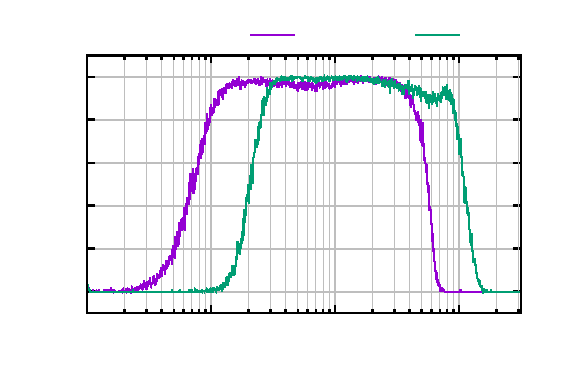
\includegraphics{pictures/freqrange}}%
    \gplfronttext
  \end{picture}%
\endgroup
}
    \caption{
        The covered frequency range for an unoptimized
        genotype $G_0$ as well as genotypes $G\ix{high}$ and $G\ix{low}$
        that are optimized for $C\ix{high}$ respectively $C\ix{low}$. Each
        of the three genotypes was tested against constant challenges
        $C_\omega$ that yielded simple sinusoidal waves with frequency
        $\omega$ for every seed value. The topology of all genotypes was
        a mere Erd�s-Renyi topology.
        The parameters for the unoptimized genotype $G_0$ were taken to be
        default values from \cite{FORCE} (which also uses Erd�s-Renyi
        topologies), while we chose genotypes $G\ix{high}$ and $G\ix{low}$
        that did particularly well when explicitly optimizing for high and
        low frequencies (see FIG. \ref{fig:freq_optimization} for more
        details).
    }
    \label{fig:freqrange}
\end{figure}


\subsection{Topology Optimizations}
To find out whether the topology can be used to improve the learning, we
performed an optimization in which the networks were an interpolation
between sparse random connections (Erd�s-Renyi) and a ring topology where
the $\RINGk$ nearest neighbors are connected (for non integer $\RINGk$, the
fractional part determines the probability to use $[\RINGk]$ or $[\RINGk]+1$).
Since we are interested in the influence of the topology, the parameters
gain and feedback are kept constant during the optimization process,
leaving the connection probability for ER topology $\ERprob$, the ring
connection length $\RINGk$ and the interpolation value $\ERtoRING$ between
ER and ring as free parameters.

The results of the optimization are depicted in FIG. \ref{}. Unfortunately,
the improvement in fitness after the first few generations in extremely
low. The development of the ration parameter, however, unambiguously shows
that the selection process prefers generators that consist mostly of ring
topology with ring parameter $\RINGk \approx 1$. The ER connection probability
shows a very broad distribution, which is simply due to the low dependence
of the generated networks on $\ERprob$ when the usage of ER topology
$\ERtoRING$ approaches zero.

\section{Discussion}
- Remarks
    * Influence of initial conditions
        -> Degenerated initial population poses major problems (does not
        find same / takes very long to find same parameters as when started
        with diversity).
        -> With broad diversity: often fast convergence -> Gen. Optimizer
        good as optimizing filter, but has hard times to explore new
        parameter regions if no right genotypes are present (especially isolated
        maxima of $F_C$). Solution: Could introduce migrants, that supply
        the gene-pool with underrepresented genotypes.
    * According to experience: maybe not ideal for finding single set of
      parameters but rather for successful parameter-ranges (branches?)


- Problems
    * Many magic / ``empiric'' parameters scattered in the model that were not examined exhaustively
    * Only few and uncomprehensive number of test / experiments conducted due to the
      computational cost.
    * Test with several other topologies did not yield concrete results,
      only rough tendencies.
    * Influence of statistics: Learning success depends stronger on choice
      of challenges than parameters (partially) -> must be very careful how to
      interpret the results / should have used fixed array of challenges instead
      of random sampling


\bibliography{sources}

\end{document}
